\documentclass[border=2pt]{standalone}
\usepackage[compat=1.1.0]{tikz-feynman}

\begin{document}
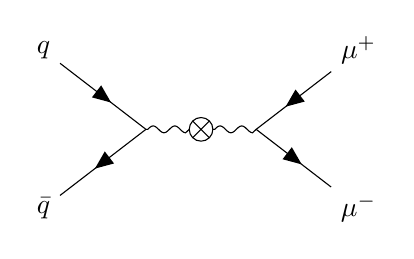
\begin{tikzpicture}
\begin{feynman}
  \vertex (q) at (0, 1) {\(q\)};
  \vertex (qbar) at (0, -1) {\(\bar{q}\)};
  \vertex (a) at (1.3, 0);
  \vertex[crossed dot] (op) at (2, 0) {};
  \vertex (b) at (2.7, 0);
  \vertex (mup) at (4, 1) {\(\mu^{+}\)};
  \vertex (mum) at (4, -1) {\(\mu^{-}\)};

  \diagram* {
    (q) -- [fermion] (a) -- [fermion] (qbar),
    (a) -- [boson] (op) -- [boson] (b),
    (mup) -- [fermion] (b) -- [fermion] (mum),
  };
\end{feynman}
\end{tikzpicture}
\end{document}
